\documentclass{article}
\usepackage[utf8]{inputenc}
\usepackage[T1]{fontenc}
\usepackage[MeX]{polski}
\usepackage{graphicx}
\usepackage[outdir=./]{epstopdf}
\usepackage{listings}

\title{%
	Implementacja i przetestowanie algorytmów \\
	dokładnych i przybliżonych \\
	dla problemów szeregowania zadań \\
	kompatybilnych na maszynach jednorodnych}
	

\author{Tomasz Wesołowski}
\date{2019}
 
\begin{document}
 
\maketitle
 
\tableofcontents
 
\section{Problem szeregowania zadań}

Szeregowanie zadań kompatybilnych na maszynach jednorodnych.

\section{Kolorowanie grafów ważonych}

Aby przejść do rozwiązywania problemu kosztowego kolorowania grafów ważonych musimy zacząć od kilku definicji formalnych. 

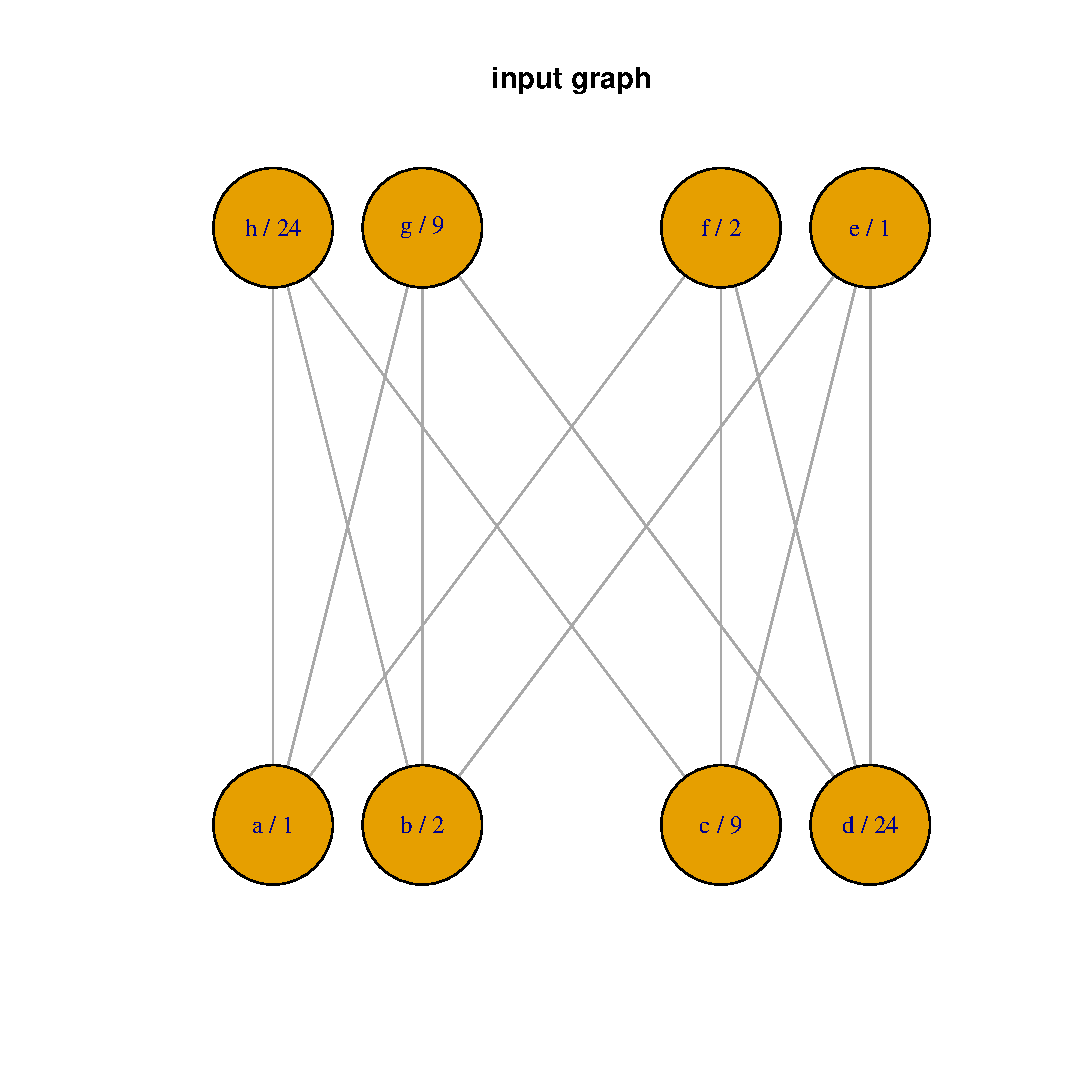
\includegraphics[scale=0.6]{graphs/reference_graph.eps}

I tak, mając graf ważony $G_w = (V,E,w)$, gdzie $V$ to zbiór wierzchołków, $E$ to zbiór krawędzi, natomiast $w$ to wagi wierzchołków takie, że  $w:V \rightarrow R_+$ oraz palete (zestaw) kolorów $C = (c_1, c_2, ..)$ taką że $\forall c_i \in N_+$ staramy się znaleźć takie przyporządkowanie kolorów do wierzchołków, by zminimalizować sumę iloczynów wag w grafie $\sum w_i * c_i = min$ oraz by żadne dwa wierzchołki mające wspólną krawędź nie miały tego samego koloru. Innymi słowy szukamy optymalnego, poprawnego kolorowania grafu.

Problem kosztowego kolorowania grafów ważonych jest problemem optymalizacyjnym, NP-trudnym. Z racji na złożoność problemu, w tej pracy zajmiemy się tylko grafami dwudzielnymi oraz weźmiemy pod uwagę tylko palety składające się z co najwyżej 4 kolorów.

\subsection{Algorytm przybliżony}

\subsubsection*{3-pseudo kolorowanie}

K-pseudokolorowaniem grafu nazywamy każde poprawne kolorowanie $k-1$ kolorami lub kolorowanie $k$ kolorami takie, że wierzchołki pokolorowane ostatnim kolorem mogą nie być niezależne, tzn. wierzchołki pokolorowane ostatnim kolorem mogą być połączone krawędziami między sobą. 

Minimalne k-pseudokolorowanie polega na takim dobraniu kolorów, by spełnione były warunki k-pseudokolorowania oraz suma iloczynów wag wierzchołków i wag kolorów była jak najmniejsza.

Algorytm polega na zbudowaniu grafu skierowanego na podstawie grafu wejściowego i wyliczeniu przecięcia S-T. W ten sposób utworzone zbiory wierzchołków, po drobnych przekształceniach, definiują 3 kolory jakimi należy pokolorować graf by otrzymać 3-pseudokolorowanie. Algorytm został znakomicie opisany w \cite{kubale-pikies19}.


\subsubsection*{27/26-przybliżony}

Algorytm 27/26-przybliżony działa w czasie $O(nm)$, ale nie gwarantuje nam znalezienia optymalnego rozwiązania. Mamy jednak pewność, że znalezione rozwiązanie nie będzie gorsze niż 27/26 rozwiązania optymalnego. 

Pierwszym krokiem jest wyznaczenie zbiorów kolorów $V1$, $V2$ oraz $V3$ poprzez algorytm minimalnego 3-pseudokolorowania. Następnie kolorujemy graf optymalnie kolorami $C1$ oraz $C2$ i obliczamy sumę kolorowania, oznaczamy ją $S1$. 

Kolejnym krokiem jest pokolorowanie kolorem $C1$ wierzchołków $V1$ które otrzymaliśmy z 3-pseudokolorowania, a pozostałą część wierzchołków kolorujemy optymalnie kolorami $C2$ oraz $C3$ i takie kolorowanie oznaczamy jako $S2$.

Następnie kolorujemy $V1$ kolorem $C1$, $V2$ kolorem $C2$, a pozostałe wierzchołki kolorujemy optymalnie $C3$ oraz $C4$ i takie pokolorowanie oznaczamy jako $S3$.

Najlepsze z pokolorowań $S1$, $S2$ oraz $S3$ (kryterium jest minimum sumy kolorowania) jest naszym rozwiązaniem. Co więcej, jest rozwiązaniem nie gorszym niż 27/26 rozwiązania optymalnego jak zostało dowiedzione w \cite{kubale-pikies19}.

\subsubsection*{Wstępna selekcja grafów łatwych}

Grafy banalne do wyliczenia optymalnego wyniku możemy łatwo zidentyfikować już na początku algorytmu. W takich przypadkach optymalne rozwiązanie uzyskujemy już w pierwszym kroku algoytmu imamy pewność że kolejne kroki nie polepszą wyniku, więc algorytm można przerwać wcześniej.

By to osiągnąć, po obliczeniu optymalnego kolorowania dwoma kolorami należy obliczyć najcięższy zbiór niezależny. Jeśli suma wag wierzchołków wyznaczonych przez ten zbiór, oraz suma wag wyznaczonych przez któryś z kolorów z dwukolorowania są sobie równe, oznacza to że osiągneliśmy wynik optymalny.

\subsection{Algorytm siłowy}

Algorytm siłowy "brute-force" polega na wygenerowaniu wszystkich możliwych sekwencji kolorów dla danego grau.. Następnie z wszystkich prawidłowych kolorowań wybieramy to, które ma najmniejszą sumę kolorowania. Ilość wszystkich kombinacji wynosi $n^k$, gdzie $n$ to ilość wierzchołków grafu, a $k$ to ilość różnych kolorów - w naszym przypadku 4.

Sposób przypisania kolorów do wierzchołków w danej sekwencji definiuje wzór $c = (x \div k^{i-1}) \bmod k$, gdzie $c$ to index koloru, $i$ to index wierzchołka w grafie, $x$ to numer danej sekwencji a $k$ ilość dostępnych kolorów w palecie. 

Sprawdzenie, czy kolorowanie jest poprawne czy nie jest banalne i polega na odwiedzeniu wszystkich wierzchołków w dowolnej kolejności oraz sprawdzeniu, czy dany wierzchołek nie ma sąsiada w tym samym kolorze co on. 

Algorytm możemy więc podzielić na 3 części - 1) wygenerowanie wszystkich możliwych kombinacji, 2) sprawdzenie każdej z nich, 3) połączenie wyników.

\subsubsection*{Optymalizacje}

Algorytm jest stosunkowo łatwy do zrównoleglenia, ponieważ pierwsza i ostatnia faza są proste obliczeniowo, natomiast w przypadku fazy środkowej (najbardziej wymagającej obliczeniowo) każdą z kombinacji może liczyć niezależnie osobny wątek.



\section{Porównanie algorytmów}

\section{Analiza wyników}

\begin{thebibliography}{9}

\bibitem{kubale-pikies19}
Tytus Pikies, Marek Kubale,
\emph{Cost coloring of weighted bipartite graphs}
(2019)

\bibitem{igraph-r}
\emph{https://igraph.org/r/doc/}

\end{thebibliography}

\end{document}
